
\subsection{Relative muon rates due to the detector geometry}

To find out whether this hypothesis is valid, it is important to know what relative rates one would expect due to the geometry of the detector and the trigger setup only. For this a Monte Carlo simulation was made. It is assumed here, that the arrival directions of the muons are isotropically from above. This is a reasonable assumption, because to be detected the muons have to come from low zenith angles anyway and nonisotrosopy only plays a significant role for high zenith angles, since there muons have to travel a longer distance through the atmosphere, which reduces their number. \\
If you had a flat detector (so only one of the three detector planes), the muonflux $mf$ for a certain zenith angle can be calculated as
\begin{equation}
  mf\left(\theta\right) = \int\cos^2\theta\mathrm{d}\theta = \frac{\theta}{2}+\frac{1}{4}\sin(2\theta)
\end{equation}
The probability for a muon to be detected also depends on the intersection area of the top and the bottom plane as seen from the muon. This is illustrated by Fig.~\ref{f:intersection}. 
  \begin{figure}[H]
    \centering
    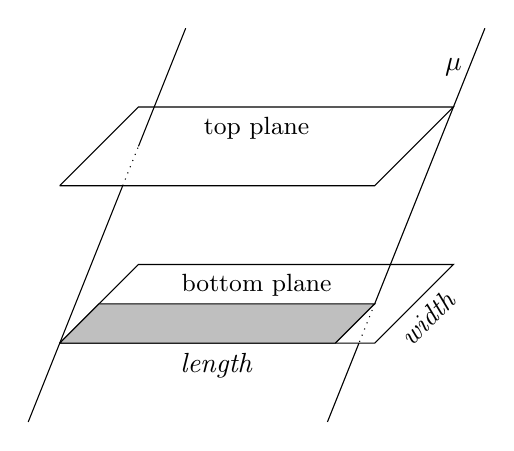
\begin{tikzpicture}
    \draw (0,0) -- (1,1) -- (5,1) -- (4,0) -- (0,0);
    \draw (0,2) -- (1,3) -- (5,3) -- (4,2) -- (0,2);
    \draw (5.4,4) -- (4,0.5);
    \draw [dotted] (4,1/2) -- (9.5/2.5 , 0);
    \draw (9.5/2.5,0) -- (3.4,-1);
    \draw [fill=lightgray] (0,0) -- (0.5,0.5) -- (4,0.5) -- (3.5,0) -- (0,0);

    \draw (-1/2.5, -1) -- (0,0) -- (2/2.5, 2);
    \draw [dotted] (2/2.5, 2) -- (1, 2.5);
    \draw (1,2.5) -- (4/2.5,4);

    \node at (5,3.5) {$\mu$}; 
    \node [below] at (2.5,3) {\small{top plane}};
    \node [below] at (2.5,1) {\small{bottom plane}};
    \node [below] at (2,0) {\textit{length}};
    \node [below, rotate=45] at (4.5,0.5) {\textit{width}};
\end{tikzpicture}

    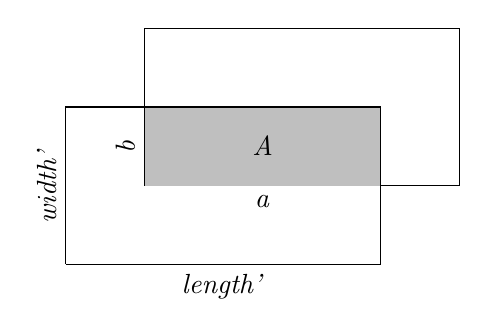
\begin{tikzpicture}
    \draw (0, 0) -- (0,2) -- (4,2) -- (4,0) -- (0,0);
    \draw (1,1) -- (1,3) -- (5,3) -- (5,1) -- (1,1); 
    \draw [fill=lightgray] (1,1) -- (1,2) -- (4,2) -- (4,1);
    \node [below] at (2,0) {\textit{length'}};
    \node [above, rotate=90] at (0,1) {\textit{width'}};
    \node [below] at (2.5,1) {\textit{a}};
    \node [above, rotate=90] at (1,1.5) {\textit{b}};
    \node at (2.5,1.5) {\textit{A}};
\end{tikzpicture}    
    \caption{\emph{Top:} side view of projected plane intersection. \emph{Bottom:} plane intersection as seen from a certain direction.}
    \label{f:intersection}
  \end{figure}
  This area can be calculated as
  \begin{align}
    a =& length - heigth\left|\sin\phi\right|\tan\theta,
  \\
    b =& width - heigth\left|\cos\phi\right|\tan\theta,
  \\
  A\left(\theta,\phi\right) =& \begin{cases}
  ab; & \text{for $a>0$ and $b>0$},
  \\
  0; & \text{otherwise},
  \end{cases}
  \end{align}
  Last but not least one has to take into account the detection efficiencies $e$ of the detector planes. Since an event is only saved if a signal is detected in the first two scintillators, the efficiency for these has to be set to 1. For the other planes the measured value is taken. 
  The expected rate of the measurement in the $n$th scintillator is therefore proportional to
  \begin{equation}
    r\propto mf\left(\theta\right)\cdot A\left(\theta,\phi\right)\cdot e
  \end{equation}
  For the simulation isotropic values for the zenith and polar angle are generated and the measurement rate (in arbitrary units) is calculated for the different heights (distance from the top scintillator to the scintillator of interest) and therefore scintillators. All of these rates are added together for each of the scintillators. By dividing the rates of the top two scintillators by the rates of the other scintillators the relative rates that should be observed due to the detector geometry can be calculated. The result can be seen in Fig.\,\ref{f:relativeRates}
\begin{figure}[H]
    \centering
    \includegraphics[width=0.5\textwidth]{figures/relativeRate.pdf}
    \caption{Relative Rates}
    \label{f:relativeRates}
\end{figure}
